\chapter{Avaliação Experimental}
\label{cap:avaliacao}

Este capítulo descreve o ambiente de simulação, os cenários, a matriz experimental e
as métricas empregadas na avaliação da arquitetura do Capítulo~\ref{cap:proposta}.
Os resultados obtidos são relatados no Capítulo~\ref{cap:resultados}.

\section{Ambiente de Simulação e Pilha de \textit{Software}}
\label{sec:setup-ambiente}

Os experimentos rodam sobre ROS~2 Humble com Gazebo Fortress (Ignition Gazebo~6)
como simulador de física, interligados por \texttt{ros\_gz}. O robô é uma plataforma
de tração diferencial (\emph{inspector\_bot}) com sensor planar de distância de
$360^\circ$.

O planejamento global de caminho usa a pilha Nav2 com o planejador global
\emph{NavfnPlanner} e um controlador \textit{Model Predictive Path Integral} (MPPI)
para seguimento de caminho (modelo de movimento diferencial, frequência de controle
de $20$~Hz) sobre um mapa de ocupação \emph{estático}. A pilha Nav2 é configurada com
\textit{Adaptive Monte Carlo Localization} (AMCL), mas nestes experimentos a
transformada \texttt{map}$\rightarrow$\texttt{odom} é mantida fixa, de modo que a
pose do robô é exata e a deriva de localização não é modelada; a pose usada pelos nós
de percepção e de métricas é, portanto, a transformada verdadeira no referencial do
mapa, e não uma estimativa do AMCL.

Os \textit{costmaps} usam raio do robô de $0{,}25$~m, raio de inflação de $0{,}55$~m
e fator de escala de custo de $3{,}0$; a tolerância de meta é de $0{,}25$~m.

\subsection{O Mundo Simulado}

O mundo modela uma subestação simplificada (Figura~\ref{fig:setup-mundo}): um
transformador de potência ($3{\times}2{\times}1{,}5$~m em $(10,10)$), um disjuntor
($1{\times}1{\times}2$~m em $(-5,5)$), um barramento
($8{\times}0{,}3{\times}0{,}3$~m em $(0,15)$) e uma cerca perimetral de
$50{\times}50$~m, sobre um plano de solo. O mapa de ocupação estático
($1040{\times}1040$ células a $0{,}05$~m/célula) é alinhado ao referencial do mundo,
de sorte que \textit{waypoints} em coordenadas do mundo servem diretamente como metas
de navegação.

A patrulha deliberativa visita cinco \textit{waypoints} (em metros): $(13,-8)$,
$(13,10)$, $(0,11)$, $(-8,5)$ e um retorno em $(-10,-10)$.

\begin{figure}[htb]
\centering
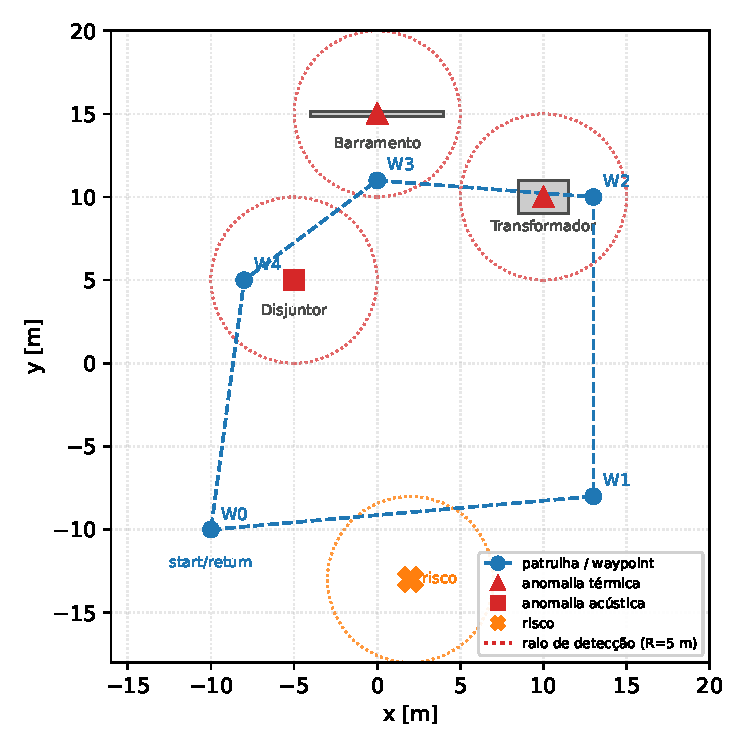
\includegraphics[width=0.85\textwidth]{figuras/world_map}
\caption{Cenário da subestação (padrão): equipamentos (cinza), os cinco
\textit{waypoints} de patrulha W0--W4 e a ronda (tracejada), as anomalias de atração
(térmica $\triangle$, acústica $\square$) e o risco ($\times$), cada qual com seu
raio de detecção $R=5$~m (pontilhado). Coordenadas em metros, referencial do mundo.}
\label{fig:setup-mundo}
\end{figure}

\section{Eventos Simulados e Cenários}
\label{sec:setup-eventos}

Conforme a Seção~\ref{sec:prop-sensoriamento}, a saída da percepção é abstraída como
eventos. Definem-se os seguintes cenários:

\begin{description}
    \item[\texttt{default}] Três anomalias de atração --- um evento térmico no
    transformador $(10,10)$, um evento térmico no barramento $(0,15)$ e um evento
    acústico no disjuntor $(-5,5)$ --- e um risco persistente (repulsão) ao lado da
    primeira perna de patrulha, em $(2,-13)$.

    \item[\texttt{adverse}] Adensa as anomalias em aglomerados (cinco anomalias: duas
    próximas ao transformador, duas próximas ao disjuntor, mais o barramento), de modo
    que múltiplos eventos caiam simultaneamente dentro do raio sensorial e a camada
    tenha de arbitrar entre eles; o risco permanece inalterado.

    \item[\texttt{route-hazard}] Mantém as três anomalias padrão mas move o risco
    \emph{para cima} da primeira perna de patrulha, em $(1{,}5,-9)$ --- bloqueando
    diretamente o caminho ao \textit{waypoint} seguinte ---, de sorte que um recuo
    puramente reativo não possa resolvê-lo sem desviar a rota. Aqui o risco detectado
    é também projetado, em sua posição \emph{percebida}, como zona de exclusão
    persistente no \textit{costmap} global.

    \item[\texttt{conflict}] Mantém as três anomalias padrão e colocaliza, na posição
    do risco padrão $(2,-13)$, uma anomalia acústica \emph{forte} ($I_e=0{,}95$,
    $|w\,I_e|=1{,}14$) com um risco \emph{mais fraco} ($I_e=0{,}70$,
    $|w\,I_e|=1{,}05$): a atração é a mais saliente das duas, de modo que uma regra
    puramente de magnitude preferiria a inspeção, ao passo que a regra de precedência
    deve disparar \textsc{Avoid}.

    \item[\texttt{dyn-hazard}] Um risco colocalizado com uma anomalia permanece
    \emph{inativo} até que o robô --- já comprometido com sua inspeção --- se aproxime
    a $3$~m, ponto em que o ambiente o ativa. É o único cenário em que o risco
    \emph{emerge} durante uma investigação.

    \item[\texttt{marginal}] Um risco de intensidade elegível mínima ao lado da
    primeira perna de patrulha, junto a uma anomalia acústica legítima de intensidade
    $0{,}95$ posicionada a $4{,}3$~m dele, para medir o custo da precedência
    categórica na faixa em que o risco governa o campo sem disparar recuo.
\end{description}

O raio de detecção é $R=5$~m, a distância de parada de inspeção é $\rho=2$~m e a
margem de recuo é $\Delta=1{,}5$~m.

\section{Matriz Experimental}
\label{sec:setup-matriz}

A camada reativa é avaliada contra uma linha de base fixa e uma linha de base de
campo potencial artificial, ao longo de uma varredura de $\eta$, de uma ablação com
$\eta=0$, de um cenário adverso, de um risco colocado sobre a rota e de perturbações
de ruído de percepção (Tabela~\ref{tab:setup-matriz}). Cada configuração é executada
$n=10$ vezes, sem interface gráfica e com limite de $600$~s por execução.

%% Acrescentado em 13/11/2026: o limite de execucao e de RELOGIO DE PAREDE, enquanto a
%% duracao de missao relatada e de relogio simulado. Sem essa distincao a KOb aparece
%% com 627 s sob um limite de 600 s, o que parece contradicao e nao e.
Esse limite é de \emph{relógio de parede} e governa o \textit{script} de execução, que
encerra o processo quando a missão não atinge o estado \texttt{COMPLETE} dentro da
janela. A duração de missão relatada no Capítulo~\ref{cap:resultados} é medida no
\emph{relógio simulado}, a partir do início da missão e já descontada a subida dos nós.
Os dois relógios não coincidem: sobre as execuções concluídas, a razão mediana entre o
relógio simulado e o de parede é de $1{,}12$ (faixa de $1{,}11$ a $1{,}15$), de sorte que
o limite de $600$~s de parede corresponde a aproximadamente $674$~s de relógio simulado,
ou cerca de $627$~s de missão. É por isso que uma configuração interrompida pelo limite
pode exibir duração de missão superior a $600$~s: o valor relatado é o do relógio
simulado no instante da interrupção, e não uma missão concluída.

\begin{table}[htb]
\centering
\caption{Matriz experimental ($10$ execuções tentadas por configuração).
\emph{Rec.} é o recuo reflexivo e \emph{ZE} a zona de exclusão deliberativa; ambos
são parâmetros de lançamento, listados aqui porque a entrega descrita na
Seção~\ref{sec:prop-keepout} só ocorre onde a zona de exclusão está habilitada. A
zona de exclusão está ligada apenas onde um risco se encontra sobre a rota de
patrulha ou emerge durante uma investigação; em todo cenário fora da rota ela está
desligada, e a reobservação pode seguir renovando o canal de risco. As linhas HEU,
HEU-sel e Q-driven abrangem três cenários cada, o que as desdobra em três rótulos de
execução; as demais correspondem a um rótulo cada. São, portanto, $32$ pares
configuração--cenário e $320$ execuções tentadas, censadas na
Tabela~\ref{tab:setup-censo}. As três linhas HAZ varrem o limiar de elegibilidade de
modalidade $\theta_{\mathcal{H}}$ (Seção~\ref{sec:res-sens-limiar}) e as duas linhas
HYS variam o par entrada/saída da histerese contra a referência $0{,}45/0{,}25$
(Seção~\ref{sec:res-histerese}); ambas as varreduras mantêm \textsc{Stay Alert} ativa
com $\eta=0{,}5$.}
\label{tab:setup-matriz}
\footnotesize
\begin{tabular}{llcccl}
\hline
\textbf{Exp.} & \textbf{Camada reativa} & $\bm{\eta}$ & \textbf{Rec.} &
\textbf{ZE} & \textbf{Cenário (\#anom./risco)}\\
\hline
E1  & nenhuma                      & ---   & ---        & ---        & \texttt{default} (3/1)\\
E0  & Stay Alert (ablação)         & 0     & \checkmark & ---        & \texttt{default} (3/1)\\
E2  & Stay Alert                   & 0,3   & \checkmark & ---        & \texttt{default} (3/1)\\
E3  & Stay Alert                   & 0,5   & \checkmark & ---        & \texttt{default} (3/1)\\
E4  & Stay Alert                   & 0,8   & \checkmark & ---        & \texttt{default} (3/1)\\
E5  & Stay Alert                   & 0,5   & \checkmark & ---        & \texttt{adverse} (5/1)\\
APF & campo potencial              & ---   & \checkmark & ---        & \texttt{default} (3/1)\\
RHM & Stay Alert                   & 0,5   & \checkmark & \checkmark & \texttt{route-hazard} (3/1)\\
RHB & nenhuma                      & ---   & ---        & ---        & \texttt{route-hazard} (3/1)\\
N1  & Stay Alert (ruído moderado)  & 0,5   & \checkmark & ---        & \texttt{default} (3/1)\\
N2  & Stay Alert (ruído alto)      & 0,5   & \checkmark & ---        & \texttt{default} (3/1)\\
CONF& Stay Alert                   & 0,5   & \checkmark & ---        & \texttt{conflict} (4/1)\\
KOa & somente zona de exclusão     & 0,5   & ---        & \checkmark & \texttt{route-hazard} (3/1)\\
KOb & somente recuo                & 0,5   & \checkmark & ---        & \texttt{route-hazard} (3/1)\\
KOF & patrulha fixa com zona excl. & ---   & ---        & \checkmark & \texttt{route-hazard} (3/1)\\
DHa & recuo $+$ zona de exclusão   & 0,5   & \checkmark & \checkmark & \texttt{dyn-hazard} (1/1)\\
DHb & somente zona de exclusão     & 0,5   & ---        & \checkmark & \texttt{dyn-hazard} (1/1)\\
HEU & supervisor heurístico        & ---   & \checkmark & ---        & \texttt{default}/\texttt{conflict}/\texttt{adverse}\\
HEU-sel & seleção por proximidade  & 0,5   & \checkmark & ---        & \texttt{default}/\texttt{conflict}/\texttt{adverse}\\
CM  & Stay Alert                   & 0,5   & \checkmark & ---        & \texttt{marginal} (4/1)\\
%% Acrescentado em 13/11/2026: bloco exploratorio de RL comportamental.
Q-driven & $Q$ greedy pre-treinada      & ---   & \checkmark & ---        & \texttt{default}/\texttt{conflict}/\texttt{adverse}\\
%% Acrescentadas em 13/11/2026: as cinco varreduras executadas e relatadas nas
%% Secoes~\ref{sec:res-sens-limiar} e~\ref{sec:res-histerese} faltavam nesta matriz,
%% embora a introducao as mencionasse e os dados existissem. Sem elas o censo de
%% execucoes nao fechava.
HAZ20 & $\theta_{\mathcal{H}}=0{,}20$  & 0,5   & \checkmark & ---        & \texttt{conflict} (4/1)\\
HAZ30 & $\theta_{\mathcal{H}}=0{,}30$  & 0,5   & \checkmark & ---        & \texttt{conflict} (4/1)\\
HAZ40 & $\theta_{\mathcal{H}}=0{,}40$  & 0,5   & \checkmark & ---        & \texttt{conflict} (4/1)\\
HYSnar & histerese $0{,}45/0{,}35$     & 0,5   & \checkmark & ---        & \texttt{default} (3/1)\\
HYSoff & histerese $0{,}55/0{,}35$     & 0,5   & \checkmark & ---        & \texttt{default} (3/1)\\
\hline
\end{tabular}
\end{table}

%% Secao acrescentada em 13/11/2026 para fechar o censo de execucoes. O problema que
%% ela resolve: a introducao declarava vinte configuracoes, a matriz listava vinte e
%% uma linhas, os dados em disco tinham trinta e dois rotulos, e a Secao 6.1.1 falava
%% de 160 tentativas -- numero correto para a matriz do artigo, nao para a desta tese.
%% Todos os totais abaixo saem do mesmo manifesto, gerado por
%% src/tese_nav/scripts/gerar_manifesto.py a partir dos CSVs e dos logs de bateria.
\section{Censo de Execuções}
\label{sec:setup-censo}

Todos os totais de execução citados nesta tese derivam de um único manifesto,
reconstruído a partir dos arquivos de métrica por execução e dos \textit{logs} de
bateria, com um registro por execução: rótulo, cenário, semente, horário de início,
desfecho do \textit{script} de execução, critério de validade, duração e arquivo de
origem. O manifesto é regenerado por \texttt{gerar\_manifesto.py} e acompanha o pacote
de reprodução.

A Tabela~\ref{tab:setup-censo} separa as quatro contagens que não devem ser somadas
entre si.

\begin{table}[htb]
\centering
\caption{Censo das execuções analisadas. O critério de validade é o de movimento
(distância percorrida $>1$~m): uma execução imóvel é um desfecho de confiabilidade de
inicialização, não um resultado de navegação, e é relatada separadamente na
Seção~\ref{sec:res-validade}. ``Interrompida pelo limite'' designa execução válida que
não atingiu \texttt{COMPLETE} dentro dos $600$~s de relógio de parede, de sorte que sua
duração é um limite inferior e não um tempo de missão.}
\label{tab:setup-censo}
\footnotesize
\begin{tabular}{lr}
\hline
\textbf{Contagem} & \textbf{Valor}\\
\hline
Pares configuração--cenário                     & $32$\\
Execuções tentadas ($10$ por par)               & $320$\\
Execuções válidas                               & $311$\\
\quad das quais concluíram a missão             & $302$\\
\quad das quais interrompidas pelo limite       & $9$ (todas KOb)\\
Execuções imóveis (falha de inicialização)      & $9$\\
Confiabilidade de partida por tentativa         & $311/320 = 97{,}2\%$\\
\hline
\end{tabular}
\end{table}

As $320$ execuções distribuem-se pelos seis cenários como $130$ em \texttt{default},
$70$ em \texttt{conflict}, $50$ em \texttt{route-hazard}, $40$ em \texttt{adverse},
$20$ em \texttt{dyn-hazard} e $10$ em \texttt{marginal}. Cada configuração usa as
sementes $1$ a $10$, uma por execução, e o manifesto registra a semente de cada uma.

As nove execuções imóveis distribuem-se por oito configurações --- APF, HEUc, HEUd,
HYSoff, KOb, N2 e RHM com uma cada, DHa com duas ---, de modo que nenhuma configuração
fica com menos de oito execuções válidas. As nove execuções interrompidas pelo limite
são \emph{todas} da configuração KOb, que não encerra a missão por construção, conforme
se analisa na Seção~\ref{sec:res-ablacao}; em todas as demais configurações, toda
execução válida atingiu \texttt{COMPLETE}.

Três contagens \emph{não} entram nesse censo, para que não sejam confundidas com
execuções da matriz:

\begin{enumerate}
    \item \textbf{Baterias anteriores descartadas.} Os \textit{logs} registram $479$
    lançamentos ao todo, contra as $320$ execuções analisadas. O excedente são baterias
    anteriores substituídas --- uma bateria contaminada por nó órfão entre execuções, um
    bloco interrompido pela metade e um ensaio de regressão para o portão de reúso ---,
    preservadas em diretórios separados em vez de apagadas. Uma execução descartada não
    é uma execução da matriz, e nenhuma delas entra em qualquer tabela de resultados.

    \item \textbf{Controles reutilizados.} Onde um bloco posterior se compara a um
    controle já executado, o controle é \emph{reutilizado}, não reexecutado: reusar um
    controle não cria execução nova. É o caso da configuração E3, que serve de controle
    do método em \texttt{default} para mais de um contraste.

    \item \textbf{Reanálises de registros existentes.} Reavaliar um limiar de métrica
    sobre os mesmos \textit{logs} --- como a reanálise do limiar de confirmação de
    inspeção da Seção~\ref{sec:res-ruido} --- é reanálise, não execução adicional.
\end{enumerate}

\section{Métricas}
\label{sec:setup-metricas}

Registram-se, por execução:

\begin{description}
    \item[Anomalias inspecionadas] Número de alvos de atração com chegada
    bem-sucedida \emph{confirmada}, no sentido da Seção~\ref{sec:prop-confirmacao}.
    Episódios encerrados como \emph{falho} ou \emph{adiado} não são contados.

    \item[Desvios de rota] Número de preempções do \textit{waypoint} corrente pela
    camada reativa. Como mostra a Seção~\ref{sec:res-custo-precedencia}, essa métrica
    é sensível à \emph{posição} do limiar de entrada, e não é contagem intrínseca do
    cenário.

    \item[Esquivas de risco (recuos)] Número de entradas no modo \textsc{Avoid}.

    \item[Distância mínima ao risco] Mínimo, ao longo da missão, da distância entre a
    posição verdadeira do robô e a posição verdadeira do risco. É medida
    independentemente de $\Phi$, de modo que suprimir o sinal reativo não a infla.

    \item[Tempo mínimo até a colisão] Mínimo da razão entre distância e velocidade
    radial de aproximação.

    \item[Colisões] Número de entradas em uma região de contato de $0{,}5$~m
    centro a centro. Com raio do robô de $0{,}25$~m configurado no planejador, essa
    distância deixa $0{,}25$~m entre a borda do robô e o ponto de risco. Trata-se de
    distância a um risco representado como \emph{ponto}; o equipamento que ele
    representa tem extensão finita, de sorte que não é afastamento de uma superfície
    física.

    \item[Tempo abaixo do afastamento] Tempo acumulado abaixo de uma faixa de $2$~m.
    Esse valor é limiar \emph{diagnóstico} adotado para medir exposição nesta
    avaliação; o estudo não declara requisito de afastamento mínimo, de modo que
    transitar abaixo dele não é violação de requisito, mas exposição que se relata.

    \item[Duração da missão e distância percorrida] Tempo total e comprimento de
    caminho até o encerramento da ronda.

    \item[Tempo de investigação] Tempo \emph{total} por execução passado em
    \textsc{Investigate}, e não média por episódio --- de modo que uma configuração
    que nunca investiga contribui com um $0$ bem definido, em vez de média
    indefinida.

    \item[Resíduo de atualização] $|\alpha\delta+\eta\Phi|$ completo, registrado como
    evidência de que os incrementos da Equação~\eqref{eq:prop-bellman} permanecem
    limitados. Conforme a Seção~\ref{sec:prop-atualizacao}, isso atesta estabilidade
    dos incrementos, não convergência nem governo do comportamento.
\end{description}

\section{Hiperparâmetros}
\label{sec:setup-hiper}

A Tabela~\ref{tab:setup-hiper} resume os hiperparâmetros do método e da simulação.

\begin{table}[htb]
\centering
\caption{Hiperparâmetros do método e da simulação.}
\label{tab:setup-hiper}
\footnotesize
\begin{tabular}{lll}
\hline
\textbf{Grupo} & \textbf{Parâmetro} & \textbf{Valor}\\
\hline
Atualização de valor & taxa de aprendizado $\alpha$ & 0,1\\
(Seção~\ref{sec:prop-atualizacao}) & desconto $\gamma$ & 0,95\\
          & peso afetivo $\eta$ & 0,3 / 0,5 / 0,8\\
          & tamanho de célula $\delta$; \textit{buckets} $B$ & 1,0~m; 4\\
          & recompensa de progresso $r_{\text{prog}}$ & 1,0\\
Campo $\Phi$ & pesos (térm./acúst./risco) & 1,0 / 1,2 / $-1{,}5$\\
          & limiares $\theta_m$ & 0,4 / 0,3 / 0,3\\
          & decaimento $\lambda$; saturação $\Phi_{\max}$ & 0,85; 2,0\\
          & período de decaimento $T_d$; resíduo $\varepsilon$ & 1~s; $10^{-3}$\\
\textsc{Stay Alert} & entrada $\theta_{\text{in}}$; saída $\theta_{\text{out}}$ & 0,45; 0,25\\
          & permanência $t_{\text{dwell}}$; orçamento $t_{\max}$ & 3~s; 40~s\\
          & refratário $t_{\text{ref}}$ & 8~s\\
Avaliador & distância de confirmação (métrica) & 3,3~m\\
Zona de exclusão & raio de projeção; raio do disco & 5~m; 1,2~m\\
Base APF  & distância de parada; orçamento & 1,8~m; 30~s\\
          & ganhos $k_{\text{att}}$/$k_{\text{rep}}$/$k_{\text{obs}}$ & 1,5 / 4,0 / 0,6\\
          & disparo; saída (magnitude de força) & 0,15; 0,08\\
          & refratário pós-recuo & 12~s\\
Eventos   & raio $R$; distância de parada $\rho$ & 5~m; 2~m\\
          & margem de recuo $\Delta$ & 1,5~m\\
\hline
\end{tabular}
\end{table}

\section{Reprodutibilidade}
\label{sec:setup-repro}

O código completo, o mundo simulado, os arquivos de lançamento, o executor de
bateria e o \textit{script} de análise estão publicamente
disponíveis\footnote{\texttt{github.com/voidmmn/tese\_react\_nav}}. \textit{Scripts}
de instalação configuram ROS~2 Humble, Gazebo Fortress e Nav2; um \textit{script} de
lote executa a matriz completa e grava um arquivo CSV por execução, e o
\textit{script} de análise produz a tabela-resumo e os testes estatísticos relatados
no Capítulo~\ref{cap:resultados}.

Os valores por execução, com sementes e desfechos individuais, são publicados junto
ao código, de modo que os denominadores de toda taxa relatada possam ser conferidos
em vez de aceitos por confiança.
